\documentclass{mpaper}

\newtheorem{theorem}{Theorem}[section]
\newtheorem{definition}[theorem]{Definition}
\newtheorem{corollary}[theorem]{Corollary}
\newtheorem{lemma}[theorem]{Lemma}

\begin{document}

\title{Counting Monochromatic Components in 2-Player Graph Burning}
\author{Lewis Dyer}
\matricnum{2299195}

\maketitle

\begin{abstract}
%very rough for now
We introduce 2-player graph burning, an extension of the graph burning process to contagion with competition. We develop multiple results on the number of monochromatic components on graph colourings resulting from 2-player graph burning.
\end{abstract}

\section{Introduction}

INTRO GOES HERE

\section{Background}

BACKGROUND GOES HERE, PROBABLY DESCRIBING GRAPH BURNING


\section{2-Player Graph Burning}
% define 2-GB formally (not sure if defining regular graph burning is needed formally?)

\subsection{Defining 2-Player Graph Burning}

First, we formalise the process of 2-Player Graph Burning on a graph $G$. Throughout, we presume that $G$ is a finite, simple, undirected graph.

\begin{definition}
\label{def/2-GB}

2-Player Graph Burning (or 2-GB for short) is a discrete-time graph process for two players. Each vertex is assigned one of 4 colours:

\begin{enumerate}
  \item \emph{White} vertices have not been burned by either player yet.
  \item \emph{Red} vertices have been burned by player 1.
  \item \emph{Blue} vertices have been burned by player 2.
  \item \emph{Green} vertices have been burned by \emph{both} players.
\end{enumerate}

At time $t=0$, all vertices are initially white. Each round consists of two main steps. First, both players simultaneously choose a white vertex, burning the vertex into that player's respective colour. Secondly, all non-white vertices, including green vertices, spread their colour onto adjacent white vertices, according to the following rules:

\begin{itemize}
  \item If a white vertex is burned by one or more vertices, all with the same colour, the white vertex is also burned with the same colour.
  \item If a white vertex is burned by both red and blue vertices, the white vertex will become green.
  \item If a white vertex is burned by either red or blue vertices (but not both), and also by green vertices, the white vertex will become red or blue, respectively. 
\end{itemize}

\end{definition}

In particular, these rules ensure that this process is symmetrical, so player 1 and player 2 can be interchanged without loss of generality.

\subsection{The cluster-counting problem}

\newcommand{\cluster}{\textsc{ClusterCounting  }}

Our main interest in this paper will be to count the maximum number of monochromatic components that can appear in any colouring of $G$ resulting from an instance of the 2-GB process. However, since we treat green vertices as being both red and blue simultaneously, defining "red monochromatic components" is somewhat ambiguous, so we modify the 2-GB process slightly to accommodate for this:

\begin{definition}
  \label{def/2-GB-modified}
  
  The \emph{red-focused} 2-player Graph Burning process is equivalent to the 2-GB process described in \ref{def/2-GB}, with the constraint that no vertices may be coloured green. Instead, if a vertex would ever be coloured green, it is coloured red instead.
\end{definition}

Throughout this paper, take 2-GB to be the red-focused 2-player Graph Burning process, unless otherwise specified.

After making this modification, we now formally define the main problem discussed:

\begin{definition}
  \label{def/cluster-counting}
  \cluster  is a decision problem determining whether a colouring with a given number of red clusters is attainable on a given graph.
  
  \begin{itemize}
      \item \textbf{Instance}: A graph $G$ and an integer $k$.
      \item \textbf{Question}: Does there exist a colouring of $G$, arising from 2-GB, such that $G$ contains at least $k$ red monochromatic components?
  \end{itemize}
  
  \cluster also refers to the corresponding optimisation problem:
  
  \begin{itemize}
      \item \textbf{Instance}: A graph $G$.
      \item \textbf{Question}: What is the largest integer $k$ such that there exists a colouring of $G$ arising from 2-GB with at least $k$ red monochromatic components?
  \end{itemize}
  
  Throughout this paper, \cluster refers to the optimisation problem, unless otherwise specified.
  
  
\end{definition}

\subsection{Burning Sequences}

We now introduce a compact notation for describing colourings which arise from 2-player graph burning:

\begin{definition}
\label{def/burning-sequence}

Given a graph $G$, a \emph{burning sequence} of length $n$, $B \in (V(G) \times V(G))^n$, is a sequence of tuples, $(r_1, b_1), (r_2, b_2), \dots, (r_n, b_n)$, such that player 1 burns vertex $r_t$ and player 2 burns vertex $b_t$ at time $t$.
\end{definition}

This sequence describes possible choices for the first $n$ rounds of the 2-GB process, but some further care is required to ensure this sequence describes valid choices for this process:

\begin{definition}
\label{def/valid-burning}

Given a burning sequence $B$, $B$ is said to be \emph{valid} if:

\begin{enumerate}
  \item For every vertex that appears in the $i^{th}$ term of $B$, say $v_i$, for every vertex in the $j^{th}$ term of $B$ such that $j < i$, say $v_j$ the distance between $v_i$ and $v_j$ is at most $(i-j)$.
  \item After the burning sequence described by $B$ is completed on $G$, every vertex is $G$ is non-white. 
\end{enumerate}

\end{definition}

From this definition, an immediate corollary is that any valid sequence in the original graph burning problem corresponds to a unique valid burning sequence in 2-player graph burning:

\begin{corollary}
\label{cor/burning-subset}

Given a valid burning sequence for the original graph burning problem, say $(v_1, v_2, \dots, v_n)$, the burning sequence $(v_1, v_1), (v_2, v_2), \dots, (v_n, v_n)$ describes a valid burning sequence in 2-player graph burning.

\end{corollary}

\subsection{Bounding the length of burning sequences}

%A useful question in the 2-player graph burning problem is to consider the maximum number of rounds required for this process to terminate, providing an upper bound for the number of valid burning sequences for a graph $G$. 
From Definition \ref{def/valid-burning}, it is clear that the size of a valid burning sequence must be bounded. Our first objective is to determine the maximum size of any valid burning sequence in a graph $G$, or equivalently the maximum number of rounds required to burn an entire graph $G$ using 2-GB.

A key heuristic when counting the maximal number of monochromatic components for a particular graph $G$ is the \emph{diameter} of $G$:

\begin{definition}
\label{def/diameter}
  Given a graph $G$ with vertex set $V(G)$, the \emph{diameter} of $G$ is given by
  
  \begin{align*}
  D(G) = \max_{u \in V(G), v \in V(G)} d(u,v)
  \end{align*}

  where $d(u,v)$ is the length of the shortest path between $u$ and $v$, and if no such path exists we say that $d(u,v) = \infty$.
\end{definition}

In the context of 2-player graph burning, this means that any instance of 2-player graph burning on $G$ will terminate within $D(G)$ rounds, when $G$ is connected. Therefore, the following bound on the maximum number of possible clusters over a connected graph $G$ is immediate:

\begin{theorem}
\label{def/diameter_bound}

For any connected graph $G$, the maximum number of red clusters attainable on $G$ is $d(G)$.

\end{theorem}

This bound is an initial example of a global bound, which can be computed by just considering the diameter of a graph. However, the following result shows that this can be easily improved for some types of graphs, namely graphs on $n$ vertices with diameter at least $\frac{n}{3}$:

\begin{theorem}
  \label{thm/connected-bound}
  For a connected graph $G$ with $n$ vertices, the maximum number of rounds required for the 2-GB process to terminate is $\lceil \frac{n}{3} \rceil$.
\end{theorem}

\begin{proof}
  Given a graph $G$, consider $U$, the subgraph induced by all white vertices in $G$. We aim to show that, if $U$ contains at least $3$ vertices, each round of 2-GB removes at least $3$ vertices from $U$.

  If $U$ contains at least $3$ vertices, then we choose $2$ vertices to initially burn, say $v_1$ and $v_2$, and we need to show that at least one other distinct vertex is adjacent to $v_1$ or $v_2$. Considering the possible degrees of $v_1$ and $v_2$ in $U$, there are two potentially problematic cases, while the other cases are straightforward.

  If $v_1$ and $v_2$ are both adjacent and have degree $1$, then no other vertices are adjacent to them. However, since $U$ has at least $3$ vertices, some other vertex $v_3$ must be in $U$, but not connected to $v_1$ or $v_2$. However, since $G$ is connected, $v_3$ must be adjacent to some non-white vertex in $G$, so $v_3$ must also be removed this round. A similar argument holds when $v_1$ and $v_2$ are both degree $0$ in $U$.
  
  %If every vertex in $U$ is of degree at least $2$, then we are done - the two chosen vertices are removed from $U$, and at least one other vertex must be adjacent to these choices, and thus is removed.
  
  %If exactly one vertex in $U$ is of degree less than $2$, then by the restriction introduced in Definition \ref{def/clusters}, one of the chosen vertices has degree at least $2$, so at least $3$ vertices will be removed from $U$ this round.

  %If $U$ contains at least two vertices of degree $1$, if they are not adjacent we are done, since their adjacent vertices will also be removed. If they are adjacent, then either they are the only two vertices remaining, or there is another vertex that is not adjacent to either vertex of degree 1. Since $G$ is connected, this other vertex must be adjacent to a vertex that is not in $U$, so thise vertex will be removed on the same round as the two other chosen vertices.

  %If $U$ contains one vertex of degree $1$ and at least 1 vertex of degree $0$, then the vertex of degree $1$ must be adjacent to a vertex of degree at least $2$, so the above case holds. 

  %If $U$ only contains vertices of degree $0$, all of these vertices will be burned this round since they must be adjacent to previously burned vertices, so if there are at least $3$ vertices in $U$ then at least $3$ vertices will be removed from $U$ this round. 

  Hence, while at least $3$ vertices remain unburned, at least $3$ vertices are burned each round, and if there are ever less than $3$ vertices remaining they will all be burned in 1 round, so the maximum number of rounds to burn all vertices is $\lceil \frac{n}{3} \rceil$.
  
\end{proof}

The following corollary shows that the bound described in Theorem \ref{thm/connected-bound} is tight, being attainable on paths:

\begin{corollary}
  \label{cor/path-clusters}

  Let $G$ be a connected graph on $n$ vertices. Then the maximum number of red clusters on $G$ is $\lceil \frac{n}{3} \rceil$, and this maximum is attainable when $G$ is a path on $n$ vertices.

\end{corollary}

\begin{proof}

Firstly, since each round can introduce at most 1 red cluster, and since the maximum number of rounds on $G$ is $\lceil \frac{n}{3} \rceil$ by Theorem \ref{thm/connected-bound}, the maximum number of red clusters on $G$ is $\lceil \frac{n}{3} \rceil$.

Now let $G$ be the path on $n$ vertices. Listing the vertices of $G$ in order from $v_1, v_2, \dots, v_n$, the burning sequence $(v_1, v_2), (v_4, v_5), \dots, (v_{n-2}, v_{n-1})$ contains $\lceil \frac{n}{3} \rceil$ red clusters.

\begin{figure}
    \centering
    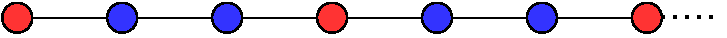
\includegraphics[scale=0.65]{mpaper/figures/PathColouring.pdf}
    \caption{An example of colouring a path, denoting $v_1$ as the leftmost vertex and so on.}
    \label{fig/path-colouring}
\end{figure}

\end{proof}

As a further example of the proof technique illustrated in Corollary \ref{cor/path-clusters}, the following lemma solves \cluster for cycles:

\begin{lemma}
\label{lem/cycle-clusters}
  Let $G$ be a cycle on $n$ vertices. Then the maximum number of red clusters on $G$ is $\lceil \frac{n}{4} \rceil$, and this bound is tight.
\end{lemma}

\begin{proof}
  Firstly, labelling the vertices of $G$ as $v_1, \dots, v_n$ in order, keeping in mind that $v_1$ is adjacent to $v_n$, the burning sequence $(v_1, v_n), (v_{n-2}, v_3), (v_5, v_{n-4}), \dots$ attains $\lceil \frac{n}{4} \rceil$ red clusters, since at each round except possibly the last, $4$ vertices are burned and $1$ new red cluster is started.

  Secondly, since every vertex has degree $2$, at least $4$ vertices must be burned every round, with the proof of this following a very similar structure to Corollary \ref{cor/path-clusters}. And since at most $1$ cluster can be created per round, the maximum number of red clusters on $G$ is at most $\lceil \frac{n}{4} \rceil$.
\end{proof}

In conjunction with Corollary \ref{cor/path-clusters}, the previous lemma presents a surprising fact: Since the maximum number of clusters on a path is $\lceil \frac{n}{3} \rceil$, and $\lceil \frac{n}{4}\rceil$ on a cycle, adding a single edge can reduce the maximum possible number of clusters on a graph by an arbitrary amount. This suggests that the diameter of a graph is an important heuristic in the \cluster problem.

\section{Colouring Caterpillar Graphs}

\subsection{Caterpillar graphs}

We now consider a natural extension of paths, and provide a method for counting clusters on these graphs.

\begin{definition}
  \label{def/caterpillars}

  A \emph{caterpillar graph} is a tree such that all vertices are within distance $1$ of some central path. We call this central path the \emph{spine}, and all vertices that are not contained in the central path are known as \emph{leaves}.
  
\end{definition}

In order to count clusters on caterpillar graphs, it will be useful to introduce more compact notation for describing caterpillar graphs:

\begin{definition}
  \label{def/caterpillar-strings}

  Given a caterpillar graph built on a spine with $n$ vertices, its \emph{caterpillar string} is a sequence $C \in \mathbb{N}^n$ of the form $(c_1, \dots, c_n)$, where $c_i$ denotes the number of leaves adjacent to the $i^{th}$ spine vertex. For instance, the caterpillar string $(1,0,2,3)$ represents the caterpillar graph shown in Figure \ref{fig/test-caterpillar-string}.
  
  \begin{figure}
      \centering
      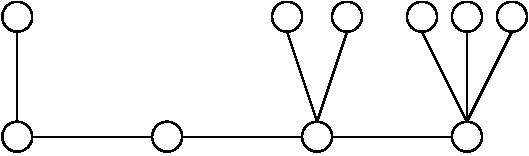
\includegraphics{mpaper/figures/testCaterpillarString.pdf}
      \caption{The caterpillar graph represented by the caterpillar string $(1,0,2,3)$. Note that reversing any caterpillar string gives an isomorphic graph.}
      \label{fig/test-caterpillar-string}
  \end{figure}
  
  

\end{definition}

Clearly, there are a countably infinite number of caterpillar strings of length $n$. However, the following lemma shows that for the purposes of \cluster we only need to consider a finite set of strings representing caterpillars.

\begin{lemma}
  \label{lem/reduced-caterpillars}

  Given a caterpillar string $C$, the maximum number of red clusters attainable in $C$ via 2-GB is equal to the maximum number of red clusters attainable in the caterpillar represented by the caterpillar string:

  \begin{equation*}
  C'_i = \begin{cases}
    0 & C_i = 0 \\
    1 & C_i \geq 1
  \end{cases}
  \end{equation*}

  In other words, if a spine vertex has more than 1 leaf, any additional leaves may be disregarded. Moreover, given such a caterpillar string $C'$, if the first or last element in $C'$ is $1$, this can be removed and two zeros can be appended to the start or end of the sequence respectively, giving an equivalent caterpillar string, say $C''$. After performing these two operations, we say that $C''$ is a \emph{reduced caterpillar string}.
\end{lemma}

\begin{proof}

For the first reduction, suppose a given spine vertex $v_i$ has at least $2$ adjacent leaves. Pick two of these leaves without loss of generality, calling them $l_1$ and $l_2$, and consider the subgraph induced by $v_i$, $l_1$ and $l_2$.

\begin{figure}
    \centering
    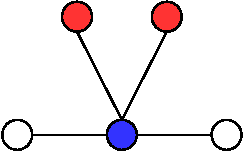
\includegraphics{mpaper/figures/CaterpillarReduction.pdf}
    \caption{In short, the proof of the first reduction is that the partial colouring presented here may never occur, and hence any given spine vertex and its associated leaves, can contain at most one red cluster.}
    \label{fig/caterpillar-reduction-1}
\end{figure}

Suppose that this subgraph contains $2$ red clusters. Then both leaves must be coloured red. However, this is only possible when $v_i$ is also red. Since both leaf vertices are not adjacent, 2 rounds are required to colour them both red, and hence the first one coloured red will spread to $v_i$, colouring it red. And if $v_i$ was already coloured blue, it would spread its colour to at least one of $l_1$ and $l_2$, so by contradiction this subgraph can contain at most $1$ red cluster. And since the leaves were chosen without any loss of generality, either no leaves are red, all leaves are red along with their common spine vertex, or exactly one leaf is red, so all but one leaf can be removed without changing the overall number of clusters.

For the second reduction, if one of the endpoints has a leaf, the leaf can be treated as a spine vertex rather than a leaf vertex, removing a leaf from the existing endpoint and becoming the new endpoint instead.
% maybe a diagram here?

\begin{figure}
    \centering
    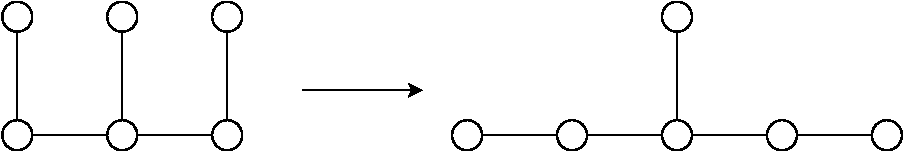
\includegraphics[scale=0.5]{mpaper/figures/CaterpillarReduction2.pdf}
    \caption{An example of the second reduction - the caterpillar with string \texttt{111} is reduced to the caterpillar with string \texttt{00100}, such that both caterpillars are isomorphic.}
    \label{fig/caterpillar-reduction-2}
\end{figure}
\end{proof}

Therefore, the set of reduced caterpillar strings of length $n$ is given by the set of bitstrings of length $n$ beginning and ending with a $0$, and hence there are $2^{n-2}$ reduced caterpillar strings of length n. In practice this may be reduced even further, since reversing the reduced caterpillar string gives another string that may be different, but which always represents an isomorphic caterpillar graph.

\subsection{Monochromatic components on caterpillar graphs}

As discussed in Lemma \ref{lem/reduced-caterpillars}, we can transform any caterpillar graph into a reduced caterpillar graph while keeping the same number of maximum red clusters on the graph. We now present the following algorithm to count the maximum number of red clusters on any reduced caterpillar graph:

Given a reduced caterpillar string, partition this string into pieces of length 3, leaving any remainder characters in the last piece which may be shorter than 3 characters, and treat each of these pieces as a (not necessarily reduced) caterpillar string.

For each of these pieces, we can easily compute the maximum number of red clusters which originate in this piece, given some starting and ending constraints. These constraints are comprised of 4 distinct cases:

\begin{itemize}
  \item In case \emph{RW}, when colouring of this piece begins, the first spine vertex is white, but the previous adjacent spine vertex, which if it exists is not part of this piece, is coloured red.
  \item Case \emph{BW} is equivalent to case \emph{RW}, except the previous spine vertex is blue instead of red. This is also the case applied for the very first piece, in order to ensure that colouring the first spine vertex red correctly counts the start of a new red cluster.
  \item Case \emph{R} is where the first spine vertex is already coloured red, since the colouring of the previous piece is not fully contained within that piece.
  \item Case \emph{B} is analogous to case \emph{R}.
\end{itemize}

\begin{figure}
    \centering
    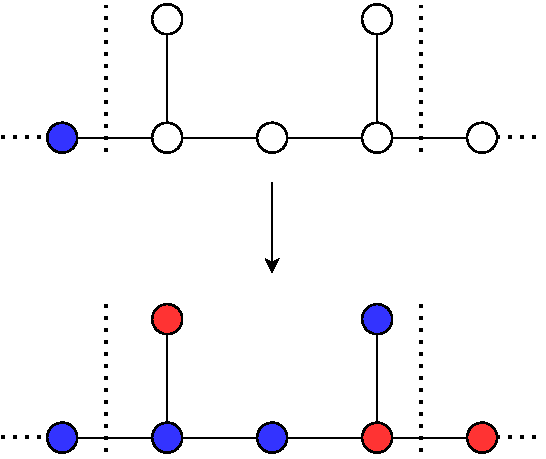
\includegraphics[scale=0.75]{mpaper/figures/CaterpillarPieceColouring.pdf}
    \caption{This figure shows the case where the caterpillar piece \texttt{101} is coloured, with starting case BW (so the previous spine vertex is already coloured blue) and ending case R (with the spine vertex after the piece being coloured red), showing that 2 red clusters are attainable in this case.}
    \label{fig/caterpillar-piece-colouring}
\end{figure}

These cases are defined for the start of a piece, but the ending constraints are analogous, and crucially correspond to the same starting constraint of the next piece.

\begin{figure}
    \centering
    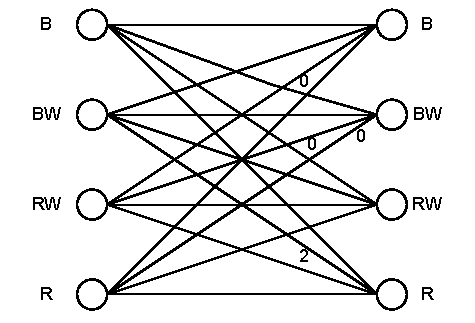
\includegraphics[scale=0.75]{mpaper/figures/ColouringGraph101.pdf}
    \caption{The bipartite graph $G_{\texttt{101}}$ representing colourings of the caterpillar graph with string \texttt{101}, with starting constraints on the left and ending constraints on the right. Note that all edges have weight 1 unless otherwise specified, and directions on edges have been omitted to improve clarity.}
    \label{fig/colouring_101}
\end{figure}

Since these pieces are small, each of these computations is small and relatively simple to perform. For each piece, this then produces a weighted directed bipartite graph $G_P$, with vertex set $\{RW_{start}, BW_{start}, R_{start}, B_{start}, \\ RW_{end}, BW_{end}, R_{end}, B_{end}\}$, such that an edge exists from $X_{start}$ to $Y_{end}$ if there exists a colouring of piece $P$ with starting constraint $X$ and ending constraint $P$, with weight equal to the number of clusters originating in $P$. An example of one of these graphs, namely $G_{\texttt{101}}$, is provided in \ref{fig/colouring-101}.

\begin{figure*}
\begin{center}
    \centering
    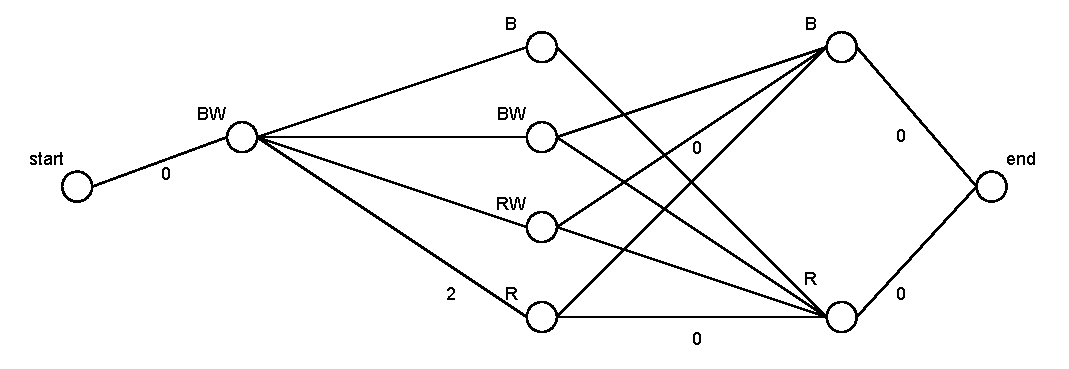
\includegraphics[scale=0.75]{mpaper/figures/Colouring_10100.pdf}
    \caption{The combined multipartite graph resulting from colouring the caterpillar with string \texttt{10100}, with unreachable vertices removed. The third layer of vertices merges together the ending constraints of piece \texttt{101} with the starting constraints of piece \texttt{00}}
    \label{fig/colouring-10100}
\end{center}
\end{figure*}

Once all of these bipartite graphs are computed, the ending vertices of each piece can be merged with the starting vertices of the next piece, along with adding in a common source and sink vertex, removing every case bar case \emph{BW} from the first piece, generating a directed acyclic multipartite graph $G$. Then, the maximum number of red clusters on the reduced caterpillar graph is equal to the length of the longest spine in $G$. An example of this combined graph, attained from colouring the caterpillar with string \texttt{10100}, is shown in Figure \ref{fig/colouring-10100}.



For future reference, we shall summarise this algorithm below:

\begin{definition}
\label{def/caterpillar-algorithm}
  Given a reduced caterpillar graph $G$, and assuming that each piece of length at most 3 has been pre-computed, a colouring for $G$ can be attained through the following algorithm:

  Partition the reduced caterpillar graph into as many connected subgraphs containing at most 3 path vertices as possible, leaving any remaining vertices in a piece at the end which may be shorter than length 3.

  For each piece, define a bipartite graph with vertices $$\{RW_{s}, BW_{s}, R_{s}, B_{s}, \\ RW_{e}, BW_{e}, R_{e}, B_{e}\}$$ such that an edge exists from $X_{s}$ to $Y_{e}$ with weight $w$ if the maximum number of red colourings originating this piece on a valid colouring with starting contraint $X$ and ending constraint $Y$ is $w$.

  After defining these graphs, define a multipartite graph $M$, merging the ending constraints of each piece and the corresponding starting constraint of the subsequent piece, along with adding source and sink vertices. Then the maximum number of red clusters on the reduced caterpillar graph is equal to the length of the longest path in $M$.
\end{definition}


Assuming that the bipartite graphs for each possible piece are pre-computed beforehand, producing the directed acyclic graph $G$ takes $O(p)$ time where $p$ is the number of pieces to combine, since each piece requires combining two constant sets of vertices together, along with constant time operations to add source and sink vertices. Since each piece adds at most $4$ additional vertices to $G$, and at most $16$ additional edges, the number of vertices and edges in $G$ are both $O(p)$. And finding the longest path in a directed acyclic graph with $V$ vertices and $E$ edges takes $O(V+E)$ time, this algorithm takes $O(p)$ time overall. But since each piece is of length at most 3, the number of pieces is linear in the length of the caterpillar, so this algorithm takes $O(n)$ time, being linear in the length of the reduced caterpillar string.


In order to justify the correctness of this method, namely that it provides the exact maximum number of red clusters attainable on $G$, we must first justifying colouring each piece in sequence.

\begin{lemma}
\label{lem/sequential-optimal}
For a (not necessarily reduced) caterpillar graph $G$ split into a series of pieces of length at most 3 as in the previous algorithm, say $P_1, \dots, P_n$, the optimal colouring in terms of maximising red clusters is attained by colouring $P_1$, then $P_2$, and so on up to $P_n$.
\end{lemma}
\begin{proof}
This proof proceeds by induction on the number of pieces in $G$.

 If $G$ has just one piece, then clearly colouring this piece will attain the optimal colouring, so the base case trivially holds.

 Now suppose the lemma holds for any (not necessarily reduced) caterpillar graph consisting of at most $n-1$ pieces. Then $G$, a caterpillar graph with $n$ pieces, is made up of the concatenation of two caterpillar graphs - one graph with $n-1$ pieces, followed by one piece.

If either end piece is fully coloured first, the lemma holds from the inductive hypothesis. If a different piece is fully covered first, then $G$ is split into two smaller graphs, each with length less than $n-1$ pieces. If an optimal colouring for one of these graphs is attained using the inductive hypothesis, then the colouring will spread to the other piece, so it is not possible to colour each of these pieces sequentially - and hence, this colouring cannot be better than the optimal colouring, so the lemma holds in this case.

Now suppose the first piece coloured is not fully covered, so another piece starts being coloured before the first piece is finished. Then the possible colourings on this first piece are a subset of all possible colourings, so the number of red clusters on this first piece cannot be any better than optimal. Then applying the inductive hypothesis to the remaining pieces means that the result holds.

\end{proof}

Note that this lemma holds for caterpillar graphs even if they are not fully reduced - in particular, their strings need not start or end in a $0$. This allows induction to be applied, since concatenating non-reduced caterpillar graphs can still lead to a reduced caterpillar graph.

The algorithm being exact follows from this lemma, since the multipartite graph constructed during the algorithm describes all possible ways to colour the caterpillar graph sequentially, and since the longest path is chosen the most optimal way to colour the whole graph is chosen, even if this means deviating from the greedy approach.

\section{Colouring Trees}
\label{sec/trees}

Compared to our previous work on paths and caterpillar trees, trees present some unique challenges when counting monochromatic components. In particular, our strategies for colouring paths and caterpillar trees generally rely on being able to limit the spread of vertices, and proceed through the graph in a clear sequence. However, in general trees do not possess a convenient start or end point, so such a sequence is not so clear to find. As a result, rather than the exact results in previous sections, we focus on approximate results for trees, improving on our existing upper bounds. Our first aim is to provide some sort of sequence to a tree, and we start by using that all trees contain a caterpillar graph:

\begin{definition}
  \label{def/maximal-caterpillar}
  Given a tree $T$, the \emph{maximal caterpillar of $T$}, denoted $C_T$, is the subgraph induced by all vertices in the longest path in $T$, along with all vertices which are distance $1$ from said path. If there are multiple longest paths in $T$, the maximal caterpillar of $T$ is induced by the path such that the number of vertices in the caterpillar is maximised.
\end{definition}

Once this caterpillar has been obtained, this can be coloured to attain an initial bound on red clusters for $T$:

\begin{corollary}
  \label{cor/tree-caterpillar}
  Given a tree $T$, the maximum number of red clusters on $T$ is at least as many as the maximum number of red clusters on $C_T$.
\end{corollary}

\begin{proof}
  Consider the colouring on $C_T$ generated by our previous procedure - we claim this colouring can also be applied when $C_T$ is a subgraph of $T$. Every vertex in $T \setminus C_T$ is adjacent to at most one vertex in $C_T$, since being adjacent to more than one vertex would result in a cycle. Therefore, these vertices are only coloured when their adjacent vertex in $C_T$ is already coloured, so the colouring of $C_T$ is unaffected by these vertices.
\end{proof}

A natural suggestion is that the tightness of this bound depends on how many vertices of $T$ are included in the maximal caterpillar, which is discussed further in the following lemma:

\begin{lemma}
  \label{lem/ratio-tends-to-zero}
  For any tree $T$, denote the \emph{caterpillar ratio of $T$} as the number of vertices in $M_T$ divided by the number of vertices in $T$. This ratio can be arbitrarily close to zero.
\end{lemma}

\begin{proof}
Let $B_h$ be the perfect binary tree with height $h$. Then the longest path on $B_h$ is obtained by travelling between a leaf node in the left subtree of the root and a leaf node in the right subtree of the root, and this path has length $2h+1$. This path has $2(h-1)$ internal nodes, and each internal node has 2 children, with one child being included in the longest path and the other child being included in the maximum caterpillar, so the number of vertices in $M_{B_h}$ is equal to $4h-1$.

However, the number of vertices in $B_h$ is $2^{h+1}-1$, so the caterpillar ratio of $B_h$ is $\frac{4h-1}{2^{h+1}-1}$, which tends to $0$ as $h$ tends to $\infty$.
\end{proof}

%idea: find the longest path in the tree, take all vertices that are distance 1 away to find a caterpillar, consider remaining vertices

This shows that, while colouring the maximal caterpillar gives a lower bound on the maximum number of red clusters in a tree $G$, an arbitrarily large proportion of the graph is not contained within the maximal caterpillar. Hence, colouring the remainder of $G \setminus C_T$ will be key to obtaining a tighter lower bound on the maximum number of red clusters in $G$.

We first remark that $G \setminus C_T$ must be disconnected, since otherwise $G$ would contain a cycle. In particular, $G \setminus C_T$ is comprised of a set of connected components that are all trees, so we define $G \setminus C_T := F$ to denote that this subgraph is a forest. Our next aim will be to understand the structure of $F$, and how this structure can be exploited to improve our bounds on the maximum number of red clusters in $T$.

\subsection{Colouring forests induced by a maximal caterpillar}
\label{sub/colouring_forests}

To begin, each tree in $F$ is adjacent to exactly one burned vertex - if it were adjacent to two or more burned vertices, this would define a cycle. We now use this fact to define some additional characteristics of each tree in $F$:

\begin{definition}
\label{def/roots}

Given a tree $T$ in $F$, a subgraph of a graph $G$ induced by a maximal caterpillar $C_G$, the \emph{root} of a tree, denoted $r_T$, is the vertex which is adjacent to a vertex on $C_G$. The root is \emph{red-adjacent} if this vertex is red, with an analogous definition for a \emph{blue-adjacent} root. In addition, the \emph{size} of $T$ is given by: $$s(T) = 1 + \max_{v \in V(T)} d(r_{T},v)$$, 
 

\end{definition}

From these definitions, it is apparent that, without choosing any vertices in $T$ to burn, any tree $T$ will be fully burned in $s(T)$ rounds. As a corollary to this, the maximum number of clusters originating in $T$ is at most $s(T)$. This provides an initial upper bound on the maximum number of red clusters in the graph $G$:

\begin{corollary}
\label{cor/root-diameter-bound-1}
Consider a partial colouring of $G$ as produced by the above procedure, and the forest of unburned vertices $F$ comprised of a set of trees $\mathcal{T}$. Then the maximum number of red clusters on $F$ is at most $$\max_{T \in \mathcal{T}} s(T)$$
\end{corollary}

Since this bound only considers the maximum size of any tree, this can allow for significant simplification when considering many trees in a forest, particularly for small size. For instance, if every tree has size $1$, then every tree will be fully burned after 1 round. Therefore at most 1 cluster can be created, so as long as at least one tree has a blue-adjacent root.

Since the caterpillar in $G$ was chosen to be maximal, this also imposes additional constraints on the size of trees in $F$. This constraint relies on the underlying caterpillar providing a sequential structure to the tree, as described in the following definition:

\begin{definition}
\label{def/tree-distance}
Given a tree $G$ with a maximal caterpillar $C_G$, denoting the endpoints of the caterpillar as vertices $s$ and $e$, the \emph{caterpillar distance} of any leaf vertex $v$ on $C_G$, denoted $cd(v)$, is equal to the length of the shortest path from $v$ to an endpoint of the spine of $C_G$, minus 2.
\end{definition}

We mark that subtracting 2 from the caterpillar distance is necessary in order to removepOnce this notion of distance to a caterpillar endpoint is defined, the maximal nature of this caterpillar implies constraints on the size of trees in the resulting forest $\mathcal{F}$:

\begin{lemma}
\label{def/tree-size-constraint}

For each tree $T$ in a forest $\mathcal{F}$ induced by the maximal caterpillar $C_G$, the rooted distance of $T$ is at most $cd(r_T)$.

\end{lemma}

If this constraint does not hold for some tree $T$, then the longest path in the tree $G$ would travel through $T$, so our caterpillar $C_G$ would not be maximal.

An important subtlety in this lemma is that the caterpillar distance of a vertex is only defined for leaf vertices on $C_G$. If there existed a tree in $G \setminus C_G$, rooted to some spine vertex $v$ in $C_G$, then any vertices in the tree adjacent to $v$ could be added to $C_G$ as leaf vertices, contradicting that $C_G$ is maximal, so any such tree must be rooted to a leaf vertex.

Combining this lemma with Corollary \ref{cor/root-diameter-bound-1}, along with the maximal distance from a spine vertex to a caterpillar endpoint, gives another key bound for the number of clusters in $\mathcal{F}$:

\begin{theorem}
\label{thm/root-diameter-bound-2}

Consider a partial colouring of $G$ as produced by the above procedure, with a maximal caterpillar of length $L$ (hence $G$ has diameter $L$), and the forest of unburned vertices $F$ comprised of a set of trees $\mathcal{T}$. Then the maximum number of red clusters on $F$ is at most $\lfloor \frac{L}{2} - 1 \rfloor$.

\end{theorem}

The main significance of this result is that the maximum number of clusters in a tree $G$ is proportional to the diameter of $G$, regardless of how many vertices are outside of the maximal caterpillar $C_G$. For example, the problem suggested in Lemma \ref{lem/ratio-tends-to-zero}, where arbitrarily many vertices may be outside of the maximal caterpillar, is mostly resolved - while the number of vertices outside of the caterpillar is unlimited, their distribution is constrained, in particular the size of the resulting trees which are formed, meaning that the number of clusters in these remaining vertices can be bounded.

Furthermore, since the maximum number of red clusters on the maximal caterpillar $C_M$ is known, the following result is an easy corollary from Theorem \ref{thm/root-diameter-bound-2}:

\begin{corollary}
\label{cor/diameter_bound_full}

Given a tree $G$ with diameter $L$, which is coloured by first colouring its maximal caterpillar $C_G$, the maximum number of red clusters on $G$ is at most $\frac{7(L-1)}{6}$.
\end{corollary}

\begin{proof}
  As previously discussed, a caterpillar of length $n$ has at most $\frac{2n-2}{3}$ red clusters, since any such caterpillar can be reduced to a caterpillar with at most $2n-2$ vertices by Lemma \ref{lem/reduced-caterpillars}. And Theorem \ref{thm/root-diameter-bound-2} shows that the number of red clusters on the rest of the graph outside of the maximal caterpillar of length $L$ has at most $\lfloor \frac{L}{2} - 1 \rfloor$ red clusters, and hence at most $\frac{L}{2} - 1$ red clusters, so summing these results together proves the corollary.
\end{proof}

This corollary leads to a potentially useful heuristic for the maximum number of red clusters in a tree, without performing any explicit colouring. Indeed, Corollary \ref{cor/diameter_bound_full} only requires computing the diameter of a given tree, which can be computed in O($|V|$) time. However, this method assumes that colouring the maximal caterpillar first maximises the total number of red clusters in the tree, which may not be the case.

This heuristic, however, can be improved further. In particular, this heuristic makes the assumption that the trees outside the maximal caterpillar retain the same size until the caterpillar is completed, whereas in reality vertices within these trees will start burning the round after their root is burned. Therefore, after burning a root vertex, we need to consider the minimum number of rounds to burn the remainder of the caterpillar.

\begin{corollary}
  \label{cor/min_rounds_caterpillar}
  Given a maximal caterpillar $C_G$ with length $L$, and index its spine vertices from $1$ to $L$, where vertex $1$ is coloured first when colouring a caterpillar. After colouring the leaf vertex $v$ adjacent to spine vertex $n$, the minimum number of rounds required to burn the rest of the caterpillar is at least $\lceil \frac{L-n-3}{6} \rceil + 1$.
\end{corollary}
\begin{proof}
First, since we colour a caterpillar by splitting it into pieces containing at most 3 spine vertices, and colouring this piece before colouring the remainder, then at most 3 spine vertices ahead of $v$ can be coloured - at most 2 other vertices in the same piece as $v$, and potentially one more in the next piece, if the ending constraints $B$ or $R$ are chosen. So the number of remaining spine vertices is at least $L - n - 3$.

To colour the remainder of the graph, we colour the spine vertices adjacent to the left and right endpoint of the unburned section respectively. This means that at most 6 spine vertices are burned per round, since the fire from these spine vertices can spread in both directions. This then repeats with the remaining unburned section of the spine until no spine vertices are remaining. At this point, some leaf vertices may still be unburned, but these will all be burned within one round. Therefore the minimum number of rounds required is at most $\lceil \frac{L-n-3}{6} \rceil + 1$, proving the corollary.
\end{proof}

An important remark of this corollary is that moving over one leaf vertex, going from position $n$ to position $n+1$, reduces the minimum number of rounds required by at most 1. And since the maximum rooted diameter of a tree rooted at a leaf at position $n+1$ is at most 1 more than that rooted at position $n$, the tree with maximum possible rooted diameter is still always found at the saame position as before.

From this result, Theorem \ref{thm/root-diameter-bound-2} can be updated further:

\begin{theorem}
  \label{thm/root-diameter-bound-3}
  
  Consider a partial colouring of $G$ as produced by the above procedure, with a maximal caterpillar of length $L$ (hence $G$ has diameter $L$), and the forest of unburned vertices $F$ comprised of a set of trees $\mathcal{T}$. Then the maximum number of red clusters on $F$ is at most $\lfloor \frac{7L-26}{6} \rfloor$.
  
  \end{theorem}

  Then in a similar manner, this theorem leads to updated bounds for Corollary \ref{cor/diameter_bound_full}:

\begin{corollary}
\label{cor/diameter_bound_full_2}
    % i've slipped up somewhere, since this is greater than the last bound for large enough L
Given a tree $G$ with diameter $L$, which is coloured by first colouring its maximal caterpillar $C_G$, the maximum number of red clusters on $G$ is at most $\frac{13(L-2)}{12}$.

\end{corollary}

We now move onto colouring graphs containing cycles, starting with cactus graphs.

\section{Colouring cactus graphs}
\label{sec/cactus_colouring}

First, we provide a definition for cactus graphs:

\begin{definition}
  \label{def/cactus_graphs}

  A \emph{cactus graph}, sometimes known as a cactus tree, is a connected graph where each edge is contained in at most one simple cycle. Equivalently, it is also a connected graph where each simple cycle has at most one vertex in common. 
\end{definition}

At first glance, the term "cactus tree" is somewhat counter-intuitive, since the defining feature of a tree is the absence of cycles. However, since [not quite sure how to justify this], an intuitive perspective on cactus graphs is to consider them as a tree structure of cycles, providing the key motivation for our work with cactus graphs.

In particular, our initial aim will be to find a natural method of transforming cactus graphs into trees, such that our work in Section \ref{sub/colouring_forests} may be applied. One initial suggestion is to remove each cycle by contracting all edges in the cycle, effectively shrinking down each cycle to a single point. This method will certainly produce a tree, but particularly when the cactus graph contains large cycles, this method removes the notion of distance between two vertices on the same cycle, when this distance may be significant in creating clusters on the resulting tree.

As previously discussed, one of the most important characteristics to consider when colouring a tree is the tree's diameter, so any transformation of a cactus graph should aim to preserve the graph's diameter, such that the path defining the cactus graph's diameter will serve as the spine for the resulting tree's maximal caterpillar after transformation. This operation, known as \emph{cycle folding}, is described in the following definition:

\begin{definition}
\label{def/cycle-folding}

% this needs fixing, will probably rephrase this in terms of a map?

Given a cactus graph $\mathcal{C}$, and a cycle $C$ in $\mathcal{C}$ with start vertices $s$ and an end vertex $e$, the \emph{cycle folding} of $\mathcal{C}$ with respect to $s$ and $e$ is the graph produced by the following operation:

\begin{itemize}
  \item Define $P_{s,e}$ as the shortest path between $s$ and $e$ in $C$, including both endpoints.
  \item For each vertex $v$ in $C \setminus P_{s,e}$, identify $v$ with the corresponding vertex $p$ in $P_{s,e}$ with $d(v,s) = d(p,s$).
  \item If any vertices in $C \setminus P_{s,e}$ have not been identified with another vertex, remove these vertices along with the subgraph rooted at this vertex which is not contained in $C$.
\end{itemize}

\end{definition}

Note that, since each simple cycle has at most one vertex in common, our choice of $s$ and $e$ uniquely determines the cycle to be folded, hence the notation $\mathcal{C}_{s,e}$ need not explicitly mention the cycle to be folded.

The following procedure describes a reduction from a cactus graph to a tree, by repeatedly applying cycle folding:

\begin{definition}
  The \emph{cactus reduction} of a cactus graph $\mathcal{C}$ is the tree $T$ resulting from the following procedure:

  \begin{enumerate}
    \item Determine the diameter of $\mathcal{C}$, and let $P$ be the path between the endpoints $u$ and $v$ that define the diameter.
    \item For every vertex in $P$ contained in some cycle $C$, determine the first and last vertex in $P$ contained in $C$, and label them $s$ and $e$ respectively. Perform cycle folding on $\mathcal{C}$ with respect to $s$ and $e$.
    \item For any remaining subgraphs of $\mathcal{C}$ containing cycles, perform the same procedure, fixing one of the endpoints of $P$ to the vertex that has already been mapped at a previous step.
  \end{enumerate}
\end{definition}

Our main motivation for introducing cycle folding is to transform a cactus graph into a tree while maintaining its diameter, so our next step is to check this property holds.

\begin{theorem}
  \label{thm/cactus-reduction-diameter}
Cactus reduction preserves diameter.
\end{theorem}

\begin{proof}

Throughout, take $\mathcal{C}$ to be a cactus graph, and $T$ the corresponding tree after cactus reduction.
  
First, consider the path $P$ between endpoints $u$ and $v$ defining the diameter of $\mathcal{C}$. In particular, if an edge in $P$ between two vertices, say $x_i$ and $x_{i+1}$, is not contained in a cycle, then cycle folding does not change this edge, so the distance between $x_i$ and $x_{i+1}$ is unchanged.

Now if an edge in $P$ is contained in a cycle, consider $P_{s,e}$ as in Definition \ref{def/cycle-folding}, where $s$ and $e$ are vertices in $P$ representing the start and end of the cycle respectively. Since we merge every vertex in $P_{s,e}$ with some other vertex in the cycle, the distance between $s$ and $e$ is unchanged. Therefore, after cactus reduction, the distance between $u$ and $v$ is unchanged, so the diameter of $T$ is at least $d$.

% this step is very rough at the moment, but I think it's the right idea?
Moreover, since the distance between specified endpoints in each cycle is maintained by cycle folding, it cannot be the case that any pair of vertices $x$ and $y$ move further apart after cycle folding, since no new edges are added, and vertices which were adjacent in $\mathcal{C}$ are also adjacent in $T$. Since the maximum distance between any pair of points in $\mathcal{C}$ is $d$, the diameter of $T$ is at most $d$, proving the theorem.
\end{proof}

As discussed in Section \ref{sec/trees}, when colouring trees, the optimal number of monochromatic components in a tree is closely connected to a tree's diameter. In cactus reduction, we have provided a method for transforming a cactus graph into a tree with the same diameter, allowing us to additionally exploit this connection for cactus graphs. We now aim to show the analogue to Corollary \ref{cor/tree-caterpillar}, to show that colouring the cactus reduction of $\mathcal{C}$ can be suitably extended to the whole of $\mathcal{C}$.

\begin{corollary}
\label{cor/colouring-extension}

Given a valid colouring of $T$, the cactus reduction of $\mathcal{C}$, this is also a (not necessarily complete) valid colouring on $\mathcal{C}$.
\end{corollary}

\begin{proof}
% extremely, extremely rough
Given any two vertices in $T$, $s$ and $t$ such that $d(s,t)=x$ for some $x$, the preimages of $s$ and $t$ must be at least distance $x$ apart in $\mathcal{C}$, with similar reasoning to the final part of the proof of Theorem \ref{thm/cactus-reduction-diameter}.
\end{proof}

From this corollary, we obtain an initial method for colouring a cactus graph $\mathcal{C}$:

\begin{itemize}
  \item Perform cactus reduction on $\mathcal{C}$ to obtain a tree $T$ with the same diameter.
  \item Find a maximal caterpillar $C$ in $T$, whose spine is given by a path between two vertices defining the diameter of $T$.
  \item Represent this caterpillar as a string as described in Definition \ref{def/caterpillar-strings}, and then perform caterpillar reduction as in Lemma \ref{lem/reduced-caterpillars} to obtain a reduced caterpillar string.
  \item Using the procedure described in Definition \ref{def/caterpillar-algorithm}, colour the caterpillar represented by the given reduced caterpillar string.
  \item Apply this colouring to the maximal caterpillar $C$.
  \item Apply this colouring to the tree $T$, while also using Theorem \ref{thm/root-diameter-bound-3} to bound the number of clusters on $T \setminus C$.
  \item Apply the resulting colouring to the cactus graph $\mathcal{C}$.
\end{itemize}

One initial concern with cactus reduction is the potential for information about the graph being lost. For example, given a cycle with endpoints $s$ and $e$, then two paths can be defined betweeh these endpoints within the cycle. If these paths have different lengths, folding this cycle will result in some vertices being lost. This presents a concern that cycle folding cannot find the optimal colouring of the cactus graph. However, the situation is actually even worse - even when both paths between the endpoints are the same length, an optimal solution may not arise from cactus reduction, as the following example shows:

\begin{lemma}
  Let $M$ be the maximum number of red clusters that can arise from any colouring of a given graph $G$ under the 2-GB process. Then if $G$ is a cactus graph, the maximum number of red clusters on a tree $T$ obtained via cactus reduction on $G$ may be strictly less than $M$.
\end{lemma}

\begin{proof}
  Consider $C_100$, which is a cycle graph. Without loss of generality, pick any two vertices $u$ and $v$ such that $d(u,v) = 50$, which is the diameter of $C_100$.

  If cactus reduction is performed, the resulting tree is a path on $51$ vertices. By Corollary \ref{cor/path-clusters}, the maximum number of red clusters attainable on this path is $17$. However, as shown in Lemma \ref{lem/cycle-clusters}, the maximum number of clusters attainable on $C_100$ is actually $25$.

\end{proof}

Indeed, following this example to its logical extreme, cactus reduction can lead to an arbitrarily large number of clusters being removed from the optimal number after cactus reduction. Since a cycle with $n$ vertices contains at most $\lceil \frac{n}{4} \rceil$ red clusters, and a path with $\lfloor \frac{n}{2} \rfloor$ vertices contains at most $\lceil \frac{\lfloor \frac{n}{2} \rfloor}{3} \rceil$ red clusters, then cactus reduction removes at most $\lceil \frac{n}{12} \rceil$ red clusters from this cycle.


{\bf Acknowledgments.}
Firstly, I would like to thank my supervisors - Jessica Enright, William Pettersson and John Sylvester - for their continual guidance and support throughout the project. I would also like to thank my parents, for always caring for me, and supporting my goals when I thought they could never be attained. And, last but not least, I would like to thank my girlfriend Jodie, for her never-ending love and kindness.

\bibliographystyle{abbrv}
\bibliography{example}


\end{document}